%\documentclass[handout]{beamer}
\documentclass{beamer}

\usepackage[english]{babel}
\usepackage[latin1]{inputenc}
\usepackage{textpos}
\usepackage{epstopdf}
\epstopdfsetup{update}
%\usepackage{pgfpages}
%\pgfpagesuselayout{resize to}[letterpaper,landscape]
%\usepackage{epstopdf}
%\epstopdfsetup{update}
\usepackage{pgfplots}
\usepackage{pgfbaseimage}
\usepackage{amsmath} 						%More mathematical
\usepackage{multirow}
%\usepackage[absolute,overlay]{textpos}
%\usepackage[tikz]{bclogo}
%\usepackage{etoolbox}
% listings for matlab code:
\usepackage{listings}
%\usepackage[autolinebreaks, useliterate]{mcode}
\lstset{backgroundcolor=\color[gray]{0.9}}

\usepackage{chemplants}
\usepackage{cancel}
\usepackage{graphicx}
\usetikzlibrary{math}
\usepackage{wasysym}
\usepackage{marvosym}

\usepackage{animate}

\usetikzlibrary{shapes.arrows}
\tikzset{My Arrow Style/.style={single arrow, draw=green!40!gray, very thick, fill=green!20!gray!10, anchor=base, align=center,text width=2cm,text=green!40!gray,rotate=-90,minimum width=0.5cm, inner sep=1mm, minimum height=0.5cm}}
\newcommand{\MyArrow}[2][]{\tikz[baseline] \node [My Arrow Style,#1] {#2};}

%-------------------------------------------------
% FOOTER
%
% Choose your footer style, by commenting other options:
%
%% - Clean: no footer, except of page number
\mode<presentation>{\usetheme{presentationTemplateBiomathFClean}}
%%  - Info: a fixed footer with basic presenter information
%\mode<presentation>{\usetheme{presentationTemplateBiomathFInfo}}
%%  - Section: Provide the sections and current section in the footer 
%\mode<presentation>{\usetheme{presentationTemplateBiomathFSection}}
%-------------------------------------------------


%voor de hand-outs
%\usepackage{pgfpages}
%\pgfpagesuselayout{2 on 1}[a4paper,border shrink=5mm]

\title{\LARGE Modelling and Simulation \normalsize of Biosystems}
\title{Modelling and Simulation of Biosystems}
\author[Daniel Illana]{Daniel Illana Gonz\'alez} %(daniel.illanagonzalez@ugent.be)}
\subtitle{Practicum 5: Calibration -- parameter estimation}
\date{Academic year 2024-2025}


\newcommand{\mtx}[2]
  {\left[\begin{array}{#1}#2\end{array}\right]}
\newcommand{\eqset}[1]
  {\left\{\begin{array}{rcl}#1\end{array}\right.}
\newcommand{\rbar}[2]
  {\left.#1\right|_{#2}}
\newcommand{\atwp}[1]
  {\rbar{#1}{\overline{X},\overline{U}}}

\usepackage{mdframed}

\newenvironment{opgave}[2][]{%
	\mdfsetup{%
		frametitle={%
			\tikz[baseline=(current bounding box.east),outer sep=0pt]
			\node[anchor=east,rectangle,fill=gray!40]
			{\strut #1};}%
	}
	\mdfsetup{%
		innertopmargin=10pt,linecolor=white!30,%
		linewidth=0pt,topline=true,%
		frametitleaboveskip=\dimexpr-\ht\strutbox\relax%
	}
	
	\begin{mdframed}[]\relax}{%
\end{mdframed}}



% Table of contents at the beginning of each section
%\AtBeginSection[]
%{
%  \begin{frame}
%    \frametitle{Outline}
%    \tableofcontents[currentsection]
%  \end{frame}
%}

% Title page customisation
\titlegraphic{}

\begin{document}

\frame[plain]{\titlepage}

\frame{
\frametitle{Pluto notebooks}
\large

Download the exercise notebooks for today. \vfill

\begin{itemize}
\item For this practicum, go to the Ufora submodule\\ \textbf{P5: Calibration $>$ files} \vfill
\item Download the Pluto notebooks and put them into your dedicated \texttt{modsim\_practica/P5\_calib} folder. \vfill
\item Go to your dedicated folder (cf. \texttt{modsim\_practica}) with a \textit{File Explorer}, then in this location either \vfill
\begin{itemize}
\item right click on your mouse and choose \texttt{Open in Terminal} (or something alike), or
\item write the command \texttt{cmd} in the address bar and click [\textit{Enter}].
\end{itemize} \vfill
\item Execute \texttt{julia launch\_pluto.jl} \vfill
\item Now you will be able to open and run the Pluto notebook of you choice. \vfill
\end{itemize}
}



\frame{
\frametitle{Today}
\Large
\begin{itemize}
	\item Calibration -- parameter estimation
	\begin{itemize}
	\large
	\item Maximum Likelihood Estimation (MLE)
	\item Maximum A Posteriori Estimation (MAP)
	\item Markov chain Monte Carlo (MCMC)
	\end{itemize} \medskip
	\item Example (intro notebook)
	\begin{itemize}
		\large
		\item Logistic growth model
	\end{itemize} \medskip
	\item Exercises
	\begin{enumerate}
		\large
		\item Exponential + Gompertz growth model (intro notebook)
		\item Fermenter, Monod kinetics (revisited)
		\item Irrigation model (revisited)
		\item Wastewater treatment (optimization problem)
	\end{enumerate}
\end{itemize}
}


\frame{
  \frametitle{Goals of this practicum}
  \Large
  \color{beamerstructure}
  {\begin{enumerate}
	\item Calibrating parameters using observed data %with MLE, MAP or MCMC
	\item Optimizing parameters to meet certain criteria
  \end{enumerate}
  }

\bigskip \bigskip \pause

\large
The following notebooks are the subjects for today:\medskip
\begin{itemize}
\item \texttt{calib\_intro.jl} (introduction) \medskip
\item \texttt{calib\_fermenter\_monod.jl}
\item \texttt{calib\_irrigation.jl} \bigskip
\item \texttt{optim\_wastewater\_treatment.jl}
\end{itemize}
  
  
}


\frame{
\frametitle{Calibration}

\bigskip

\centering
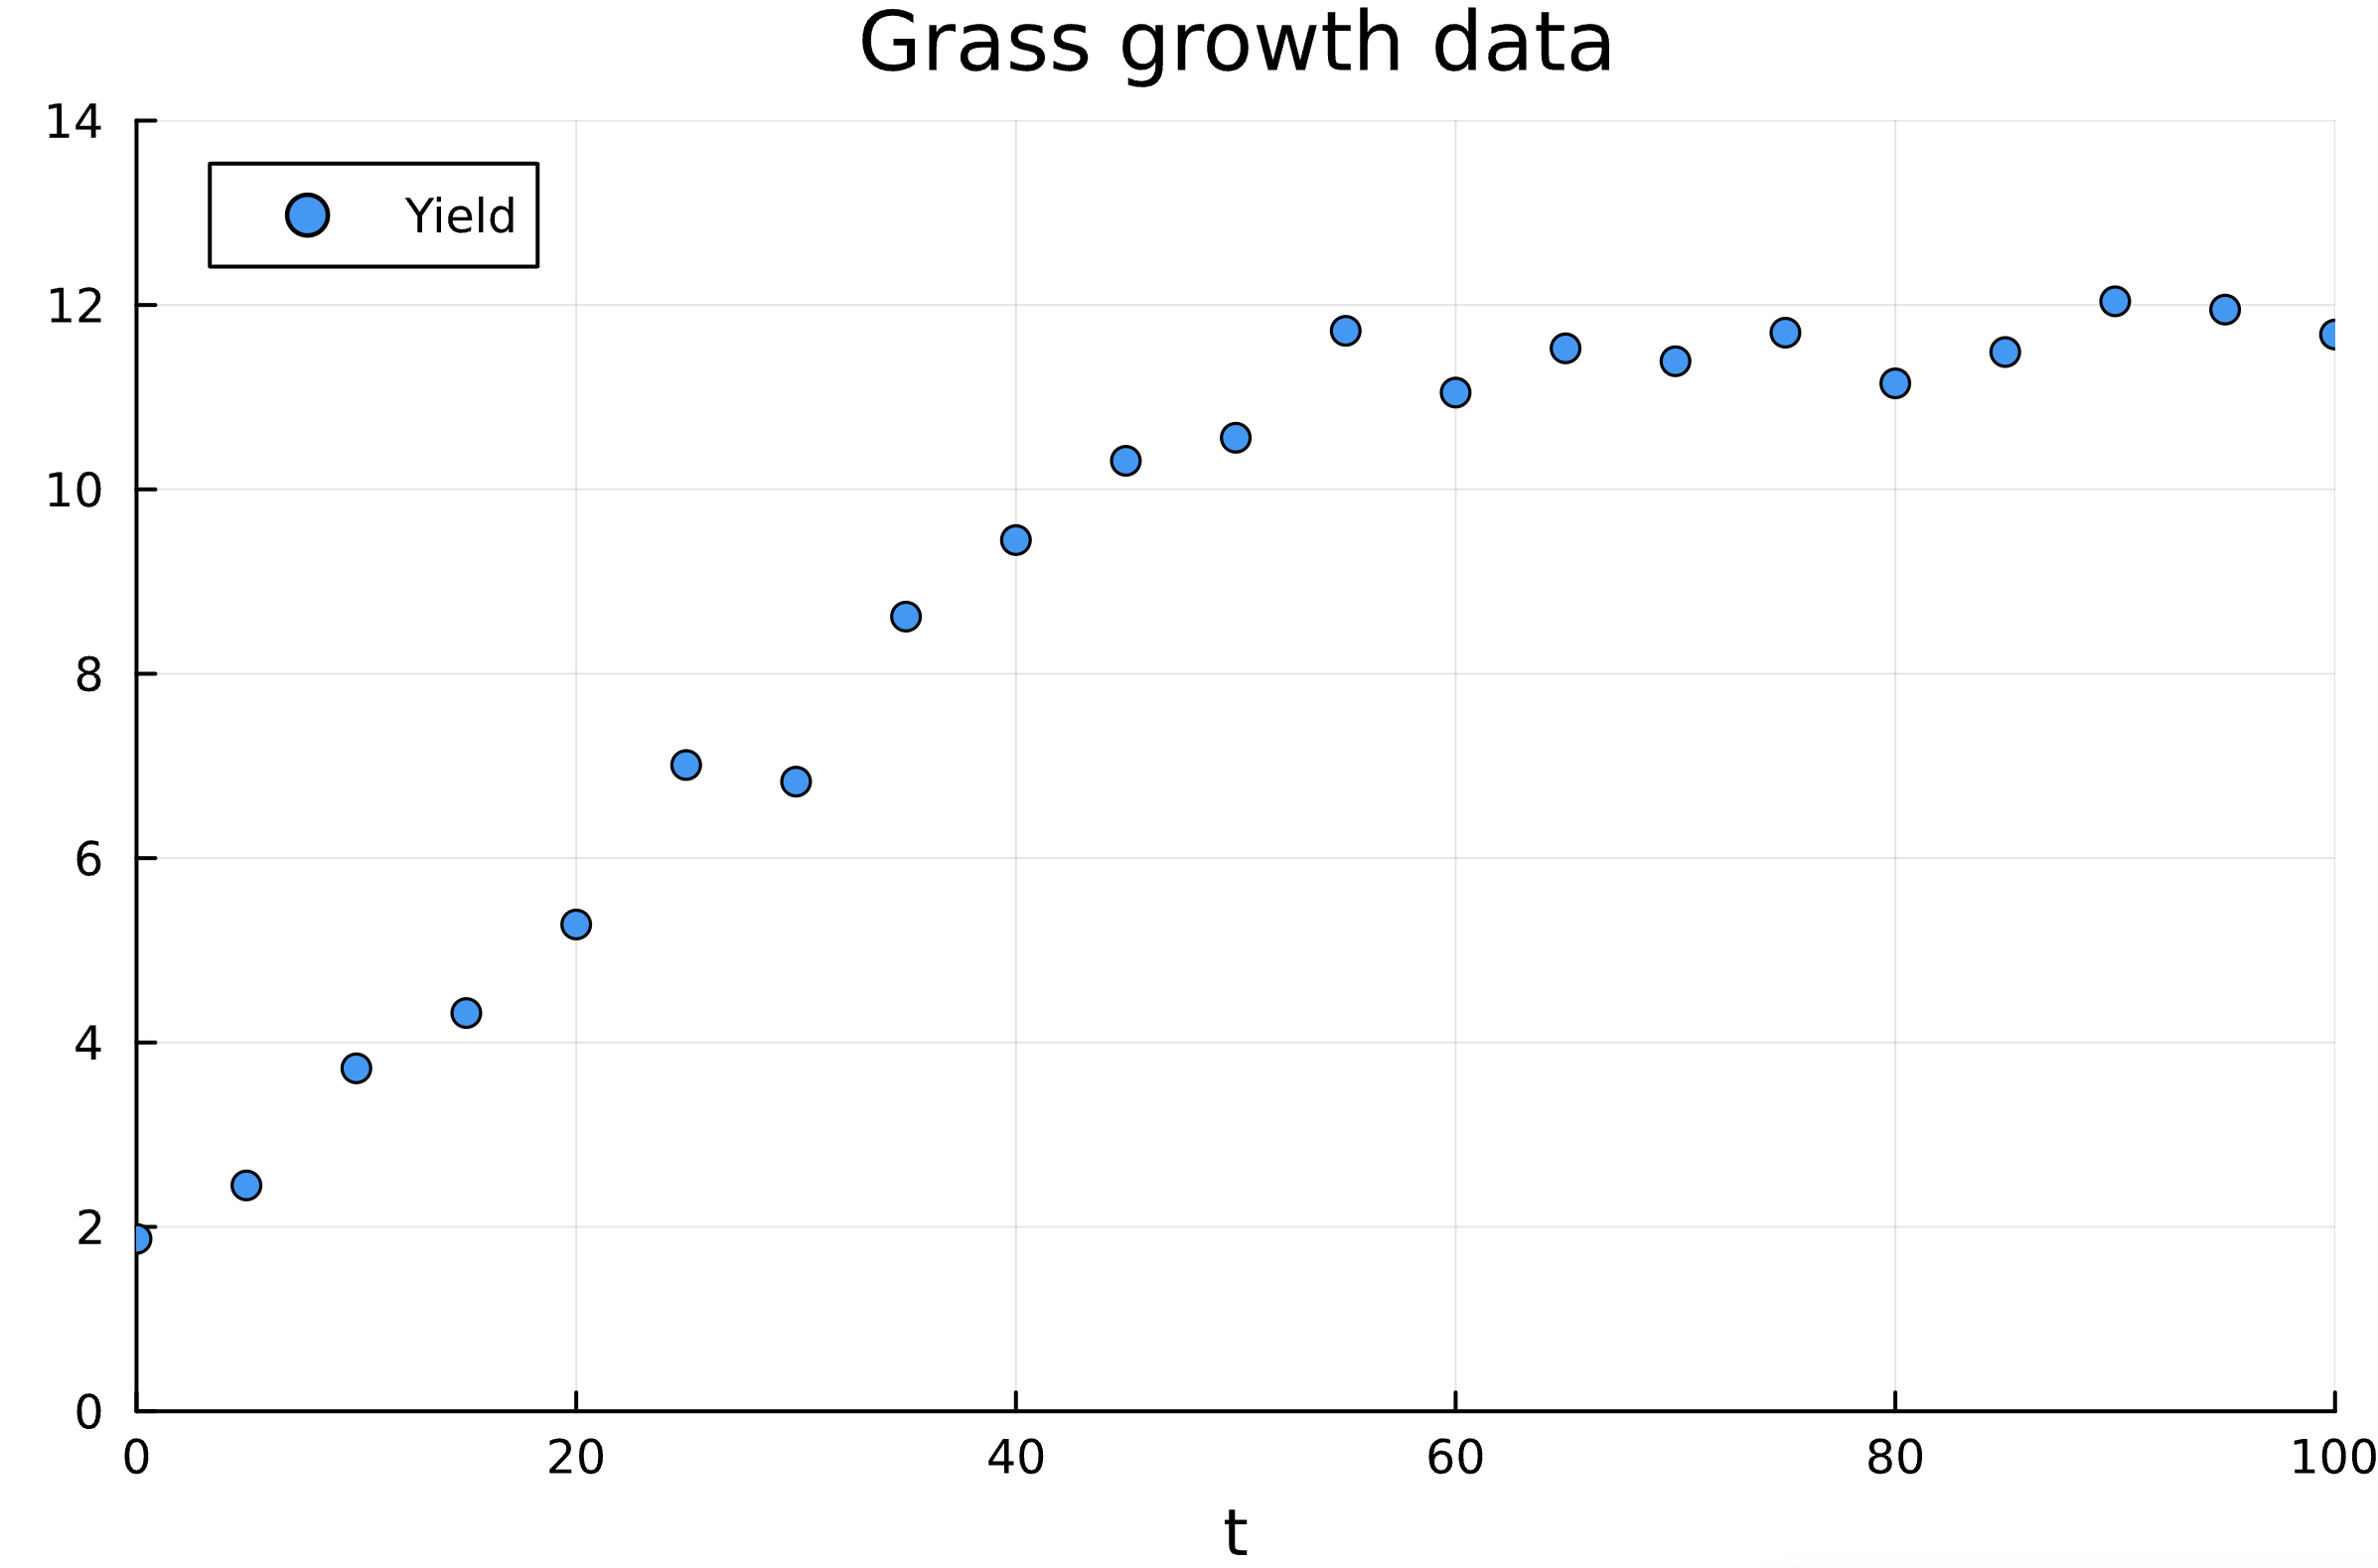
\includegraphics[width=0.9\linewidth]{figs/calibration}

\bigskip

Task: \textbf{estimate parameters from candidate model to observed data}

}





\frame{
\frametitle{Maximum Likelihood Estimation (MLE)}
\large\bigskip
\textbf{Maximum Likelihood Estimation}  is a \textbf{frequentist} method used for estimating model parameters. It finds the parameter values that maximize the (log-)likelihood of the observed data given a model.\vspace*{2mm}

Mathematically, if we denote the parameter to estimate as $\theta$ and the observed data as $D$, the MLE estimate is:

$$
\hat{\theta}_{MLE} = \arg \max_{\theta} P(D|\theta)
$$

\bigskip \normalsize

Normally-distributed errors equivalent to weighted least squares!

\bigskip \large

\begin{itemize}
\item \textbf{Intuition:} Imagine you have some data and a model with an unknown parameter. MLE asks: What value of the parameter makes the observed data most probable?
\end{itemize}



}



\frame{
\frametitle{Maximum A Posteriori Estimation (MAP)}
\large
\textbf{Maximum A Posteriori Estimation} (MAP) is a \textbf{Bayesian} alternative to MLE. It incorporates \textbf{\color{ugent-la}prior information} about the parameter $\theta$. Instead of maximizing the (log-)likelihood alone, MAP maximizes the posterior probability of the parameter given the data:
$$
\hat{\theta}_{MAP} = \arg \max_{\theta} P(\theta|D) = \arg \max_{\theta} P(D|\theta)\, \color{ugent-la} P(\theta)
$$

MAP results in a single ``best guess'' for $\theta$. \bigskip

\begin{itemize}
\item \textbf{Intuition:} Instead of only relying on the observed data (MLE), MAP takes into account what we already know or believe about parameter $\theta$ (the prior).
\end{itemize}

}


\frame{
\frametitle{Markov chain Monte Carlo (MCMC)}

\bigskip\bigskip

\large
\textbf{Markov chain Monte Carlo} (MCMC) methods are \textbf{full Bayesian} methods and come into play when we want to fully explore the posterior distribution of parameters, rather than just finding a single best estimate (like MLE or MAP). \bigskip

Instead of returning just one ``best'' estimate, Bayesian inference wants the entire posterior distribution:
$$
P(\theta|D) = \cfrac{P(D|\theta) P(\theta)}{P(D)}
$$

\pause

Summarizing:

{\scriptsize
\begin{table}
\begin{tabular}{|c|c|c|c|}
\hline
\textbf{Method} & \textbf{MLE} & \textbf{MAP} & \textbf{Full Bayesian (MCMC)} \\
\hline
\text{Returns} & $\hat{\theta}$ \text{(point estimate)} & $\hat{\theta}$ \text{(point estimate)} & $P(\theta | D)$ \text{(full distribution)} \\
\hline
\text{Prior required?} & \text{No} & \text{Yes} & \text{Yes} \\
\hline
\text{Uncertainty?} & \text{No} & \text{No} & \text{Yes} \\
\hline
%\text{Overfitting risk?} & \text{High (small data)} & \text{Lower} & \text{Lowest} \\
%\hline
\text{Computation time} & \text{Fast} & \text{Fast} & \text{Slow} \\
\hline
\end{tabular}
\end{table}
}


}

\frame{
\frametitle{Optimization}

\bigskip

\centering
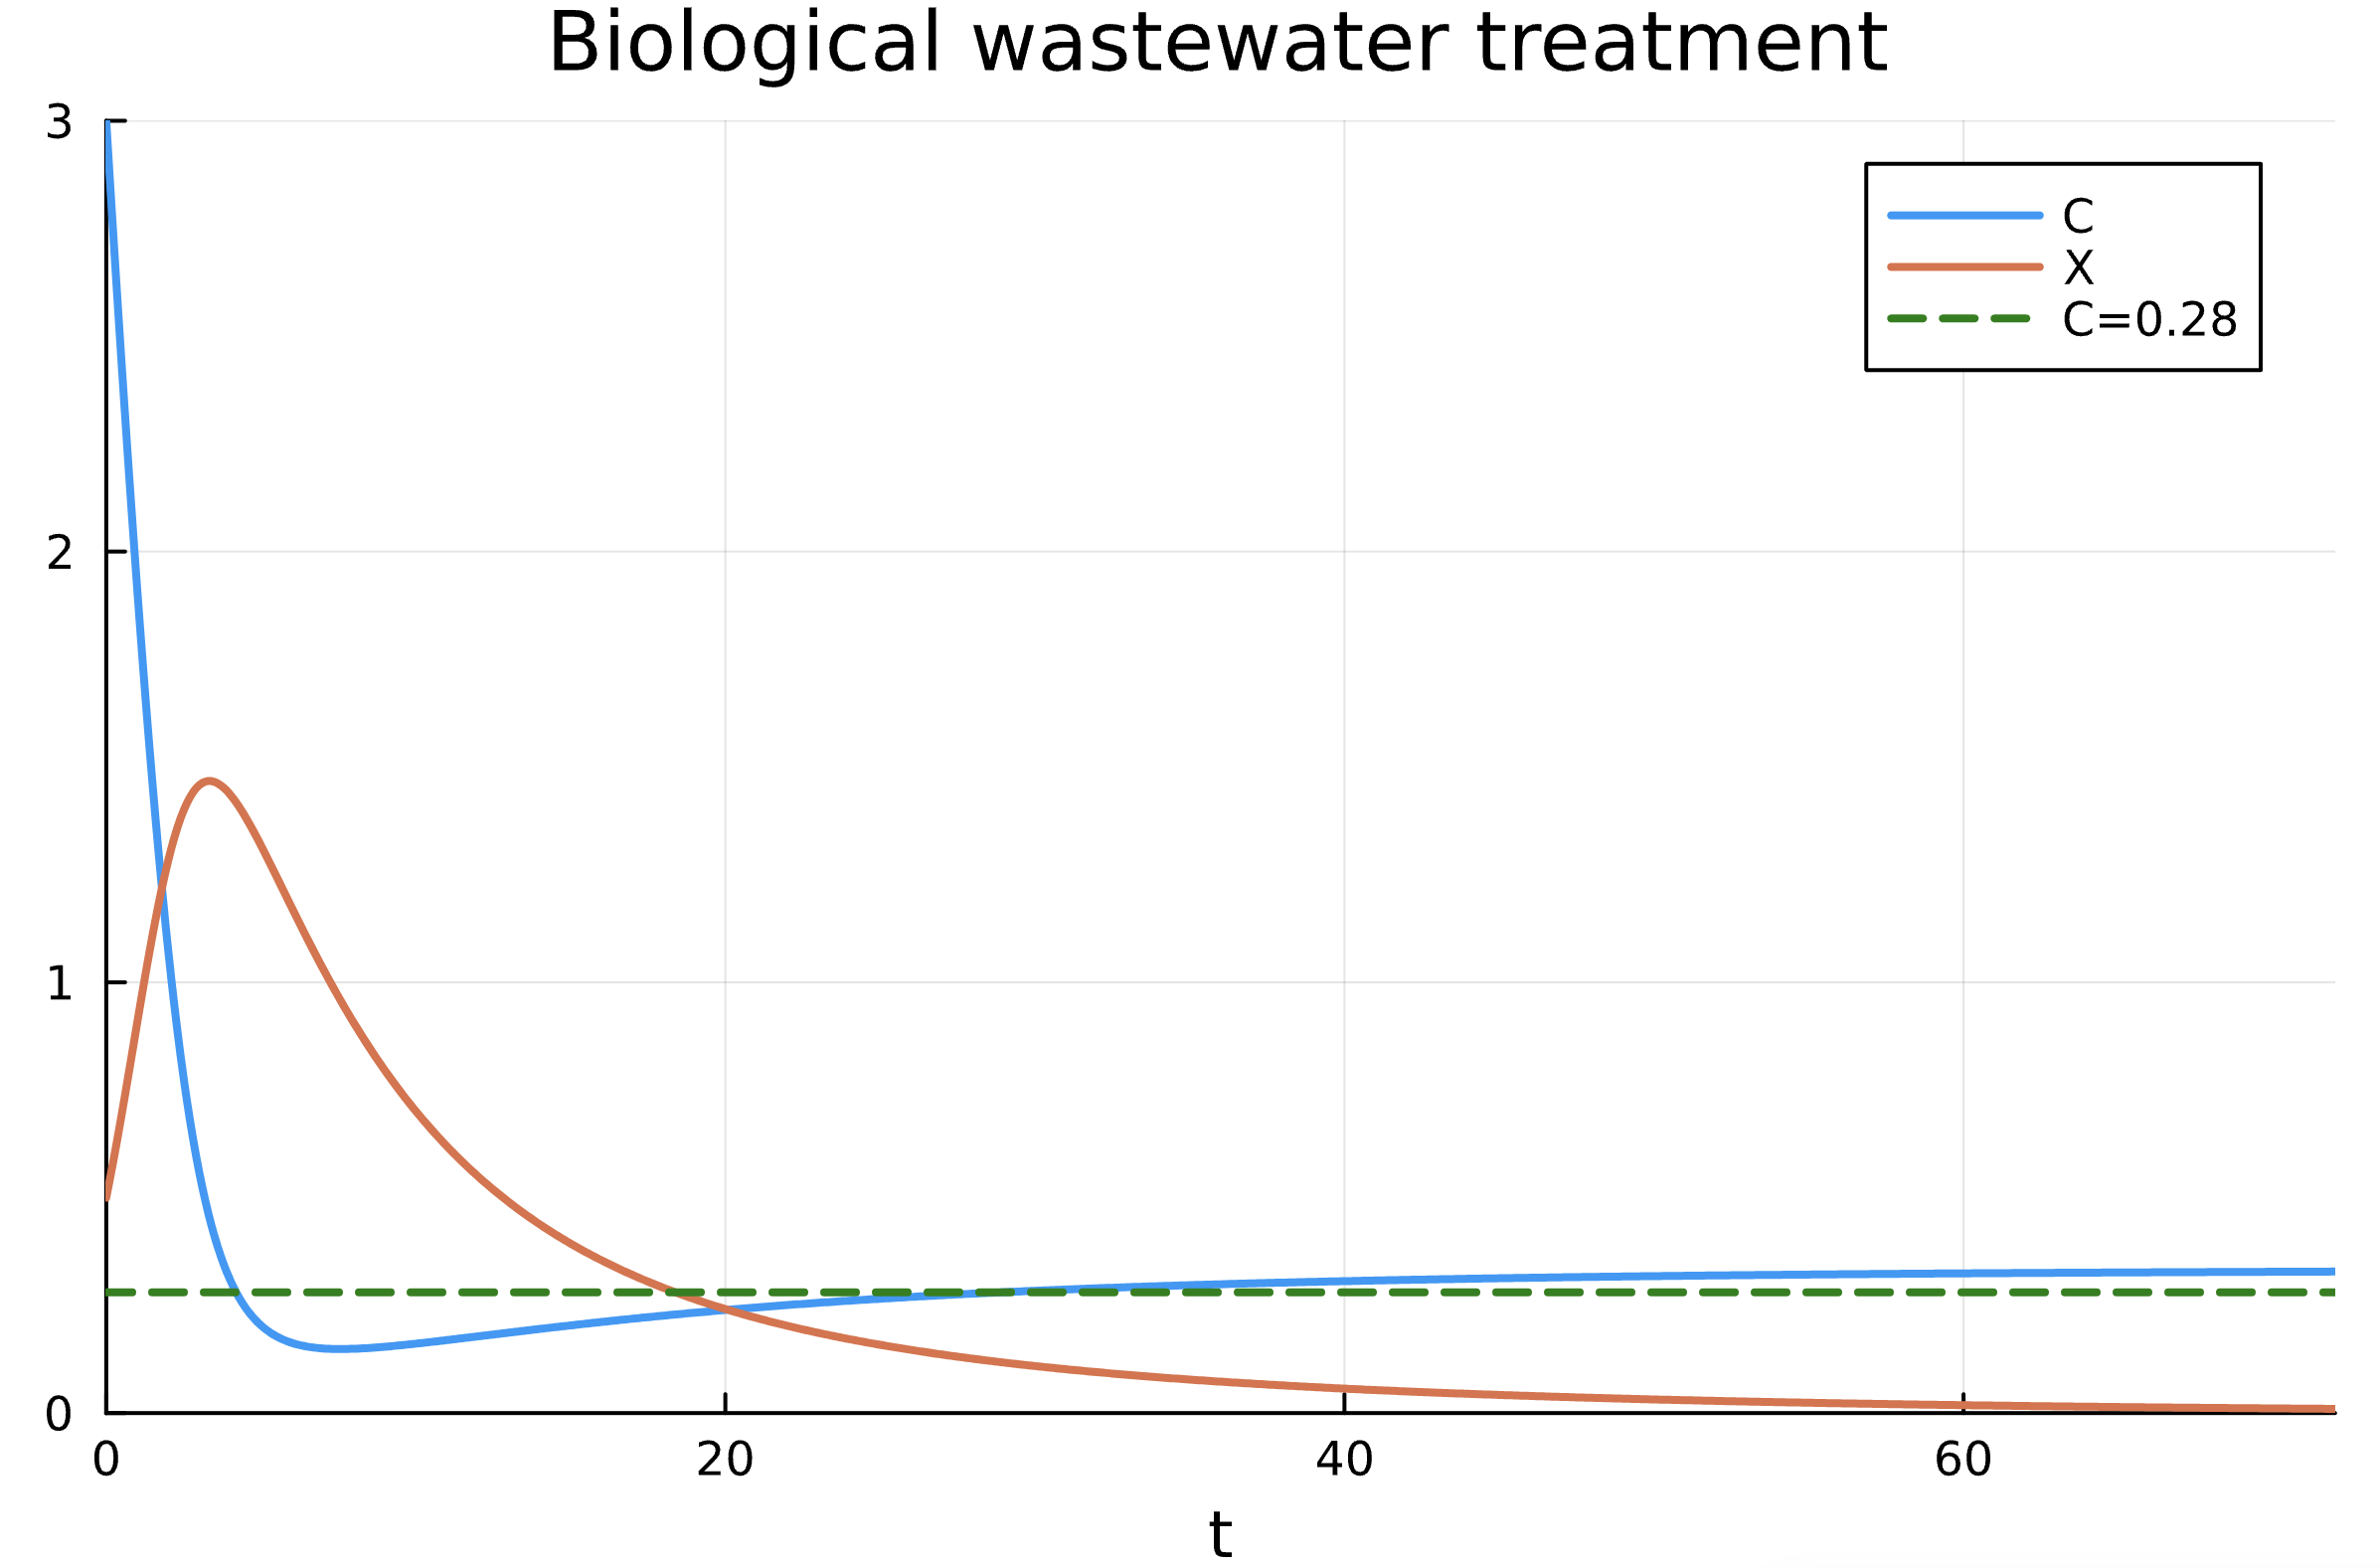
\includegraphics[width=0.9\linewidth]{figs/optimization}

\bigskip

Task: \textbf{optimize the flow rate so that organic waste is limited}

}


\frame{
\frametitle{In practice}
\large

Condition your model to the observed data (or other criteria): \medskip

\texttt{model\_cond = model({\color{ugent-la}t\_meas}) \color{ugent-la} | (Ys = Y\_meas,)} \bigskip

Use MLE or MAP and an optimization algorithm: \smallskip

\texttt{res\_mle = {\color{ugent-la}optimize}(model\_cond, {\color{ugent-la}MLE()}, NelderMead())} \\
\texttt{res\_map = {\color{ugent-la}optimize}(model\_cond, {\color{ugent-la}MAP()}, NelderMead())} \\ \bigskip

Obtain the best estimates: \smallskip

\texttt{{\color{ugent-la}coeftable}(res\_mle)} \\
\texttt{{\color{ugent-la}coeftable}(res\_map)} \bigskip

Or use MCMC to obtain the full posterior distribution: \smallskip

\texttt{res\_mcmc = {\color{ugent-la}sample}(model\_cond, {\color{ugent-la}NUTS()}, 1000)} \\ \smallskip
\texttt{{\color{ugent-la}summarize}(res\_mcmc)}


}

\end{document}

